
%%%%%%%%%%%%%%%%%%%%%%%%%%%%%%%%%%%%%%%%%%%%%%%%%%%%%%%%%%%%
\item Draw two different (that is non-isomorphic) connected graphs each having the degree sequence 3,3.2,1, 1,1, 1. \\ 
\noindent Give one reason why the graphs you have drawn are not isomorphic. 
\smallskip
%%%%%%%%%%%%%%%%%%%%%%%%%%%%%%%%%%%%%%%%%%%%%%%%%%%%%%%%%%%%
\item Let G be a simple graph. Explain why the sum of the degrees of the vertices of $G$ is twice the number of its edges.\\
\noindent Justifying your answer, say whether it is possible to construct a simple graph with degree sequence 3,3,3,3,3,3. 
\smallskip
%%%%%%%%%%%%%%%%%%%%%%%%%%%%%%%%%%%%%%%%%%%%%%%%%%%%%%%%%%%%
\item Draw two non-isomorphic graphs with the following degree sequence.
\[ 4,3,3,2,2,2,2,1,1\]
\smallskip
%%%%%%%%%%%%%%%%%%%%%%%%%%%%%%%%%%%%%%%%%%%%%%%%%%%%%%%%%%%%
\item 
\begin{enumerate}[(a)]
\item Sketch the complete graph $K_5$. What is the degree of each vertex? How many edges does it have? 
\item What is the degree of each vertex of the complete graph $K_n$? How many edges does it have? 
\end{enumerate}
\smallskip
%%%%%%%%%%%%%%%%%%%%%%%%%%%%%%%%%%%%%%%%%%%%%%%%%%%%%%%%%%%%
\item Which, if any, of the following graphs are planar graphs.
\begin{center}
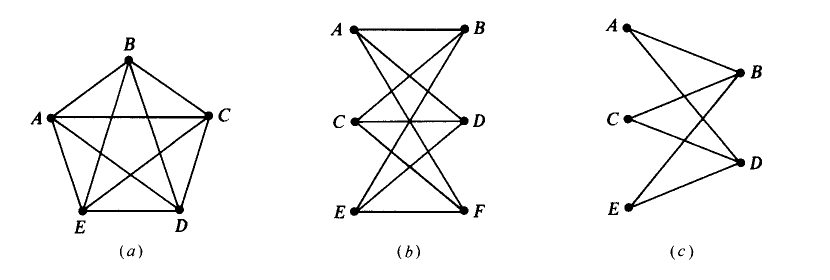
\includegraphics[scale=0.65]{Discrete-Maths-0-MASTERs/images/GraphTheory-PlanarGraphs2.png}    
\end{center}
%%%%%%%%%%%%%%%%%%%%%%%%%%%%%%%%%%%%%%%%%%%%%%%%%%%%%%%%%%%%
\item Count the number $V$ of vertices, the number $E$ of edges, and the number  of regions $R$ in
the four graphs below. For each graph, verify Euler’s formula.
\begin{center}
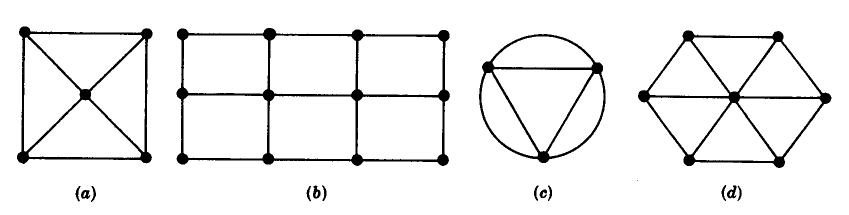
\includegraphics[scale=0.65]{Discrete-Maths-0-MASTERs/images/GraphTheory-PlanarGraphs1.png}    
\end{center}
\item State the degree of the out regions of the graphs in the previous question.
\end{enumerate}
%%%%%%%%%%%%%%%%%%%%%%%%%%%%%%%%%%%%%%%%%%%%%%%%%%%%%%%%%%%%
\end{document}